\documentclass[sigconf]{acmart}

\usepackage{booktabs} % For formal tables


% Copyright
%\setcopyright{none}
%\setcopyright{acmcopyright}
%\setcopyright{acmlicensed}
\setcopyright{rightsretained}
%\setcopyright{usgov}
%\setcopyright{usgovmixed}
%\setcopyright{cagov}
%\setcopyright{cagovmixed}


% DOI
\acmDOI{10.475/123_4}

% ISBN
\acmISBN{123-4567-24-567/08/06}

%Conference
\acmConference[WebScience'17]{ACM Web Science Conference}{June 2017}{Troy, New York, USA} 
\acmYear{2017}
\copyrightyear{2017}

\acmPrice{15.00}


\begin{document}

\title{Automated content moderation and political bias: balancing ideological diversity with civility}

\titlenote{Produces the permission block, and
  copyright information}
\subtitle{Extended Abstract}
\subtitlenote{The full version of the author's guide is available as
  \texttt{acmart.pdf} document}


\author{%
\textbf{Reuben Binns}\\
\textbf{Jun Zhao}\\
\textbf{Max Van Kleek}\\
\textbf{Nigel Shadbolt}\\
\affaddr{University of Oxford} \\
\affaddr{Oxford, United Kingdom} \\
\email{reuben.binns@cs.ox.ac.uk}} \\

% The default list of authors is too long for headers}
\renewcommand{\shortauthors}{Binns et al.}

\keywords{ACM proceedings, \LaTeX, text tagging}

\begin{abstract}
The web has become a key forum for political debate, as people take to platforms to comment and express their political viewpoints. However, online comment platforms sometimes contain abusive comments. Recent work has explored automated means of flagging abusive comments, by automatically classifying them as either toxic or civil. While such algorithmic content moderation may promote diversity by encouraging participation from those who would otherwise face abuse, it might also reproduce political biases inherent in training data, resulting in disparate impacts across partisan divides. This paper aims to better understand the potential risks of algorithmic ideological bias in such contexts. We train a simple text classifier using an existing data set of 100,000 Wikipedia comments rated by humans for 'toxicity'. This classifier is applied to a corpus of 4,000 sentences which have been labelled for ideological bias. We find that conservative sentences are more likely than liberal sentences to be automatically classified as toxic. We discuss the potential for and desirability of methods to mitigate such biases, and the implications of such systems for ideological diversity in the public sphere of the web.
\end{abstract}


\maketitle

\section{keywords} political science
algorithmic accountability
machine learning
online abuse
discussion platforms

\section{Introduction}

recent proposals suggest sanitizing online conversations using algorithmic models to classify comments as either toxic or non-toxic.

 league of legends online gaming. started on wikipedia - 63m english talk pages. wishlist.

\section{Background}

Generic work on online discussions.
"hate speech ([7], [13], [19], [27]), online
harassment ([3], [40]), and cyberbullying ([17], [20], [25], [35],
[38]).
 A recent Pew Research Center study defines online
harassment to include being: called offensive names, purposefully
embarrassed, stalked, sexually harassed, physically threatened,
and harassed in a sustained manner [5].
The Wikimedia Foundation found that
54% of those who had experienced online harassment expressed
decreased participation in the project where they experienced the
harassment [23]. Online hate speech and cyberbullying are also
closely connected to suppressing the expression of others [21], physical
violence [29], and suicide [4]""

Abuse.

lots of companies want to use machien learning to detect toxic:

perspective api - google

disqus
https://blog.disqus.com/first-steps-to-curbing-toxicity

do we want to attack the training data a bit more?

look at which words contributed to the ratings for men / women, old / young?

then look at a distance metric to show the difference between the most important words flagged by each community.

\subsection{Automated detection}

"Yin et al.’s 2009 paper [40] which used support vector machines
on sentiment and context features extracted from the CAW
2.0 dataset [6]. In [21], Sood et al. use the same algorithmic framework
to detect personal insults using a dataset labeled via Amazon
Mechanical Turk from the Yahoo! Buzz social news site. Dinakar
et al. [4] decompose the issue of cyberbullying by training separate
classifiers for attacks based on sexual orientation, race or intelligence
in YouTube comments. Building on these works, Cheng et
al. [3] use random forests and logistic regression techniques to
predict which users of the comment sections of several news sites
would become banned for antisocial behavior. Most recently, Nobata
et al. [15] extract character n-gram, linguistic, syntactic, and""Nobata et al. [15]: character-level ngrams
result in an impressively flexible and performant classifier
for a variety of abusive language in English.""
"We labeled our subset of comments using the Crowdflower crowdsourcing
platform'"

\subsection{Discovering and mitigating bias in machine learning models}
DADM and FAT-ML.

mostly concerned with fairness in terms of non-discrimination. race, gender. as yet, not applied to political diversity.


\subsection{Data sources}

\subsubsection{Wikipedia Talk Annotations}
100k annotations. toxic or not. high level of inter-annotator agreement - Krippendorf’s alpha score of 0.45".
png

\subsection{Methodology}

We began with exploratory analysis of the data.

we measued agreement within and bvetween genders.

We then trained using a dataset of manually scored comments.

we trained a classifier along the lines of the wikipedia detox project
(maybe: we also benchmarked against the jigsaw perspective API)

evaluated using the ROC / AUC.
https://en.wikipedia.org/wiki/Receiver_operating_characteristic#Area_under_the_curve

We used a bootstrapping method to sample annotators. For each comment which had both male and female raters, we selected 10 male / female annotators at random, with replacement. We then took the average toxicity/personal attack/abuse rating for these 10 sampled raters. 

used this to generate 10 different sets of training data for each gender.

These 10 different sets of training data were used to train 10 different text classifiers to identify comments that are toxic/personal attack/abuse.

We then tested these classifiers against four different sets of test data.

- previously unseen comments withheld from the detox dataset, labelled by a mixture of males and females.

- previously unseen comments withheld from the detox dataset that had been labelled by males, randomly sampled using the same bootstrap method.

- previously unseen comments withheld from the detox dataset that had been labelled by females, randomly sampled using the same bootstrap method.

-previously unseen comments from a different dataset, of twitter posts labelled 'offensive' or 'inoffensive' by a different set of crowd workers whose demographics are unknown.
% (i haven't done mixed yet, not sure its necessary).


% NB: we aren't claiming that gender is necessarily a strong determinant of norms about offense, nor are we making any claim about the origins (whether environmental, genetic or otherwise) of any putative gender differences in norms about offense, nor any normative endorsement of a particular set of norms about offense. Gender is just an easily understood and accessible demographic attribute of the labelling population, which we hypothesised would exhibit some differences between demographics. Our aim is not to essentialise gender differences. just using gender as one example of socially constructed distinction which may correlate with different norms about offence.

\section{Results}





-

structure

1. exploratory data analysis.

krippendorffs alpha - demographic subgroups differ in their judgements.
women have more diversity in what they consider offensive

2. differences in strength of coefficients between models

we compared the coefficients between the male and female classifiers. We took the features used by the classifiers, and calculated their average coefficient across the 10 classifiers created for each gender. 

3. classifier performance

-- NEW STUFF

regular classifier using the uncleaned / unbalanced training data:

normal test...
[[25506  2627]
 [  570  3163]]
 0.914089779682
test on male
[[24082  2978]
 [  696  2898]]
0.87293598743
test on female
[[23547  3513]
 [  729  2865]]
0.83643219522

---

female classifier 2
0.864523514035
[[ 2311  1035]
 [ 2160 25148]]
test on male
0.872300851164
[[ 2727   619]
 [ 3149 24159]]
test on female
0.844219435233
[[ 2706   640]
 [ 3672 23636]]
0.839958493448
[[ 876  865]
 [ 173 2033]]
computin` fairness measures...
true positive male / female: 1.00776053215
false positive male / female: 0.9671875 
false negative male / female: 0.8575708061 
true negative male / female: 1.0221272635
% female classifiers are a bit in terms of FP, a bit more in terms of FN, and roughly equal in terms of TP and TN.

male classifier 2
normal test...
0.863501899338
[[ 2292   971]
 [ 2179 25212]]
test on male
0.873261313356
[[ 2706   557]
 [ 3170 24221]]
test on female
0.839203777263
[[ 2684   579]
 [ 3694 23697]]
0.840970992782
[[ 875  917]
 [ 174 1981]]
computin` fairness measures...
true positive male / female: 1.00819672131
false positive male / female: 0.962003454231 
false negative male / female: 0.858148348674 
true negative male / female: 1.02211250369

% very similar to above. almost no difference in fairness between male and female classifiers.

male classifier 3
normal test...
0.862967752231
[[ 2298   987]
 [ 2173 25196]]
test on male
0.872288838432
[[ 2726   559]
 [ 3150 24219]]
test on female
0.838961411857
[[ 2678   607]
 [ 3700 23669]]
0.840358164238
[[ 884  915]
 [ 165 1983]]
computin` fairness measures...
true positive male / female: 1.01792382375
false positive male / female: 0.920922570016 
false negative male / female: 0.851351351351 
true negative male / female: 1.02323714563

% quite different to male 2

male classifier 4
normal test...
0.863159668303
[[ 2308   986]
 [ 2163 25197]]
test on male
0.873346103048
[[ 2740   554]
 [ 3136 24224]]
test on female
0.839641786565
[[ 2691   603]
 [ 3687 23673]]
0.840823624458
[[ 888  918]
 [ 161 1980]]
computin` fairness measures...
true positive male / female: 1.0182088443
false positive male / female: 0.918739635158 
false negative male / female: 0.850556007594 
true negative male / female: 1.0232754615

-


and 'fairness'

% explanation of the error rate comparison: we ask 'how well does this classifier do in a world where offense is defined by women, compared to a world where offense is defined by men?'. the comparison between error rates can be used to define a gender-specific notion of classifier 'fairness'. If a classifier performs worse according to female-defined offense, than it does compared to male-defined offense, it can be said to be 'unfair to women' in the sense that it is worse at tracking their collective judgements about offense.



% so looks like both male and female-trained classifiers have a higher error rate on female-labelled test data than male-labelled test data. In other words, both are 'unfair' to women, in the sense that they are worse at replicating women's collective judgements about offense than men's. However, the male-trained classifiers have a higher disparity in type I error rates between female vs male-labelled test data than female-trained classifiers. in other words, compared to bots trained by women, bots trained by men are more likely to mis-classify comments that women think are inoffensive as offensive. Both male and female-trained bots are worse at capturing women's collective judgements about offense than men's; but for male-trained bots, the disparity is greater.

As established in the previous section, the female raters broader divergence in labelling probably explains why the classifiers are generally worse at predicting female labels.

\section{Discussion}

we then discuss the significance of our findings.

the consequences go deep into methodological questions in political philosophy.

maybe the crowd-workers’ notions of toxicity are partisanal?
but maybe lib / con are just more offensive?

first, can toxicity be separated from partisanship in a way which does not beg the question?
second, what is the right amount of diversity in a free society?
How can we get past biases in the training data?

to this end, we re-trained the model using only demographic subsets of the crowd-workers (gender, age, education). These alternative models yielded differential disparate impacts on partisan groups. (to test their significance, we also trained multiple randomly drawn subsets to obtain an expected observation for the null hypothesis).

potential partisan bias mitigation strategies (sub-class of discrimination-aware data mining).

\subsection{Future work}

\section{Conclusions}

\begin{figure}[h!]
\begin{center}
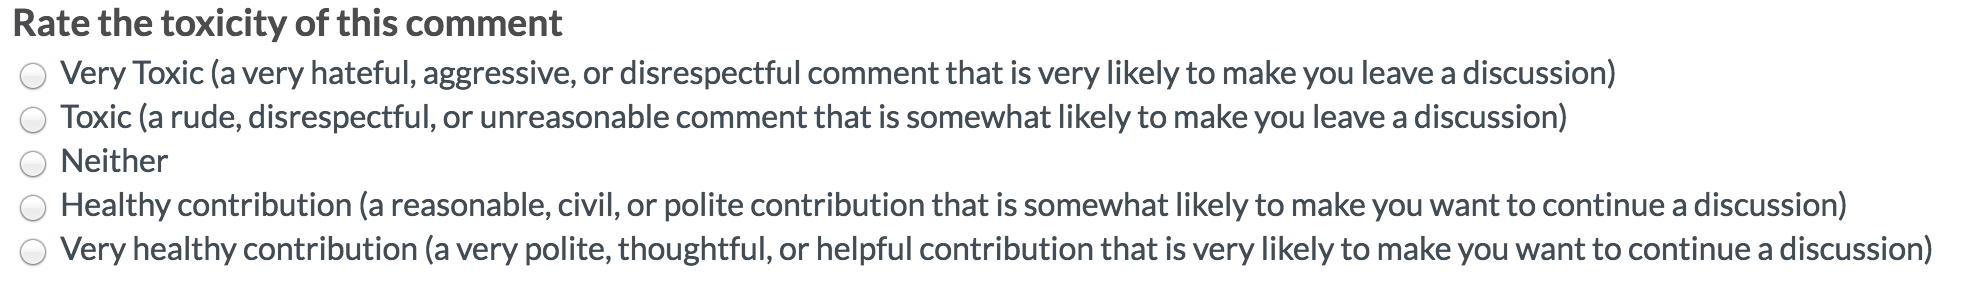
\includegraphics[width=\columnwidth]{figures/toxicity_question.png}
\caption{blah blah}\label{fig:method}
\end{center}
\end{figure}


% Bibliography
\bibliographystyle{ACM-Reference-Format}
\bibliography{acmsmall-sample-bibfile,websci-2017}

\medskip


\end{document}
% End of v2-acmsmall-sample.tex (March 2012) - Gerry Murray, ACM


